\documentclass[12pt]{article}

\usepackage{amssymb,amsmath,amsthm}
\usepackage[top=1in, bottom=1in, left=1.25in, right=1.25in]{geometry}
\usepackage{fancyhdr}
\usepackage{enumerate}
\usepackage[bw,framed,numbered]{mcode}
\usepackage{graphicx}

% Comment the following line to use TeX's default font of Computer Modern.
\usepackage{times,txfonts}

\newtheoremstyle{homework}% name of the style to be used
  {18pt}% measure of space to leave above the theorem. E.g.: 3pt
  {12pt}% measure of space to leave below the theorem. E.g.: 3pt
  {}% name of font to use in the body of the theorem
  {}% measure of space to indent
  {\bfseries}% name of head font
  {:}% punctuation between head and body
  {2ex}% space after theorem head; " " = normal interword space
  {}% Manually specify head
\theoremstyle{homework} 

% Set up an Exercise environment and a Solution label.
\newtheorem*{exercisecore}{Exercise \@currentlabel}
\newenvironment{exercise}[1]
{\def\@currentlabel{#1}\exercisecore}
{\endexercisecore}

\newcommand{\localhead}[1]{\par\smallskip\noindent\textbf{#1}\nobreak\\}%
\newcommand\solution{\localhead{Solution:}}

%%%%%%%%%%%%%%%%%%%%%%%%%%%%%%%%%%%%%%%%%%%%%%%%%%%%%%%%%%%%%%%%%%%%%%%%
%
% Stuff for getting the name/document date/title across the header
\makeatletter
\RequirePackage{fancyhdr}
\pagestyle{fancy}
\fancyfoot[C]{\ifnum \value{page} > 1\relax\thepage\fi}
\fancyhead[L]{\ifx\@doclabel\@empty\else\@doclabel\fi}
\fancyhead[C]{\ifx\@docdate\@empty\else\@docdate\fi}
\fancyhead[R]{\ifx\@docauthor\@empty\else\@docauthor\fi}
\headheight 15pt

\def\doclabel#1{\gdef\@doclabel{#1}}
\doclabel{Use {\tt\textbackslash doclabel\{MY LABEL\}}.}
\def\docdate#1{\gdef\@docdate{#1}}
\docdate{Use {\tt\textbackslash docdate\{MY DATE\}}.}
\def\docauthor#1{\gdef\@docauthor{#1}}
\docauthor{Use {\tt\textbackslash docauthor\{MY NAME\}}.}
\makeatother

% Shortcuts for blackboard bold number sets (reals, integers, etc.)
\newcommand{\Reals}{\ensuremath{\mathbb R}}
\newcommand{\Nats}{\ensuremath{\mathbb N}}
\newcommand{\Ints}{\ensuremath{\mathbb Z}}
\newcommand{\Rats}{\ensuremath{\mathbb Q}}
\newcommand{\Cplx}{\ensuremath{\mathbb C}}
\newcommand{\Aut}{\ensuremath{\text{Aut}}}
%% Some equivalents that some people may prefer.
\let\RR\Reals
\let\NN\Nats
\let\II\Ints
\let\CC\Cplx

%%%%%%%%%%%%%%%%%%%%%%%%%%%%%%%%%%%%%%%%%%%%%%%%%%%%%%%%%%%%%%%%%%%%%%%%%%%%%%%%%%%%%%%
%%%%%%%%%%%%%%%%%%%%%%%%%%%%%%%%%%%%%%%%%%%%%%%%%%%%%%%%%%%%%%%%%%%%%%%%%%%%%%%%%%%%%%%
% 
% The main document start here.

% The following commands set up the material that appears in the header.

%%%%%%%%%%%%%%%%%%%%%%%%%%%%%%%%%%%%%%%%%%%%%%%%%%%%%%%%%%%%%%%%%%%%%%%%%%%%%%%%%%%%%%%
%%%%%%%%%%%%%%%%%%%%%%%%%%%%%%%%%%%%%%%%%%%%%%%%%%%%%%%%%%%%%%%%%%%%%%%%%%%%%%%%%%%%%%%
% 
% The main document start here.

% The following commands set up the material that appears in the header.
\doclabel{Abstract hw 8}
\docauthor{Parker Whaley}
\docdate{March 3 2017}
%\lstinputlisting{}
\newcommand{\vv}{\mathbf{v}}
\begin{document}
\begin{exercise}{7.10}
Give an example of a group $G$ and subgroups $H$ and $K$ such that $HK$ is not a subgroup of $G$.\\
Define $G=S_3$.  Define $H=\{e,(12)\}$ and define $K=\{e,(13)\}$.  Note that $H$ and $K$ are subgroups of $G$.  Note that $HK=\{e,(12),(13),(132)\}$ is not a group since $(13)(12)=(123)\not\in HK$.
\end{exercise}

\begin{exercise}{7.11}
If $H$ and $K$ are subgroups of $G$ and $g$ belongs to $G$, show that $g(H \cap K) = gH \cap gK$.\\
Suppose $a\in g(H \cap K)$.  Note that there exists some $b\in H \cap K$ such that $a=gb$.  Note that $b\in H$, thus $gb\in gH$ and $b\in K$, thus $gb\in gK$, thus $a=gb\in gH \cap gK$.  We see that $g(H \cap K) \subseteq gH \cap gK$.\\
Suppose $a\in gH \cap gK$.  Note that $a\in gH$, thus there exists some $b\in H$ such that $a=gb$.  Note that $a\in gK$, thus there exists some $c\in K$ such that $a=gc$.  Note that $b=g^{-1}a=c$ thus $b\in K$.  Note that $b\in H \cap K$, thus $a=gb\in g(H \cap K)$.  We conclude $g(H \cap K) = gH \cap gK$.
\end{exercise}

\begin{exercise}{7.18}
Recall that, for any integer $n$ greater than $1$, $\phi(n)$ denotes the number of positive integers less than $n$ and relatively prime to $n$. Prove that if $a$ is any integer relatively prime to $n$, then $a^{\phi(n)} \mod n = 1$.\\
Note that $a\in U(n)$.  Note that $|a|\mid |U(n)|=\phi(n)$.  Note that $k|a|=\phi(n)$ for some integer $k$.  Note that $a^{\phi(n)} \mod n$ is the same as $a^{\phi(n)}$ in $U(n)$.  Note that $a^{\phi(n)}=a^{k|a|}=e^k=1$.
\end{exercise}

\begin{exercise}{7.22}
Suppose $H$ and $K$ are subgroups of a group $G$. If $|H| = 12$ and $|K| = 35$, find $|H \cap K|$. Generalize.\\
Note that $H \cap K$ is a group.  Note that $H \cap K<H$ and $H \cap K<K$.  Note that $|H \cap K|\mid |H|$ and $|H \cap K|\mid |K|$.  Note that $12=2\cdot 2\cdot 3$ and $35=5\cdot 7$ are relatively prime thus the only positive common denominator is $1$ thus $|H \cap K|=1$.\\
Note that what was done above works as long as $|H|$ and $|K|$ are relatively prime.
\end{exercise}

\begin{exercise}{7.26}
Suppose that $G$ is a group with more than one element and $G$ has no proper, nontrivial subgroups. Prove that $|G|$ is prime. (Do not assume at the outset that $G$ is finite.)\\
Note that for any $a\in G-\{e\}$, $<a>$ is a non-trivial sub-group of $G$, thus $<a>=G$.\\
Suppose $G$ is infinite.  Note that all non-identity elements must be generators of $G$ and thus have infinite order.  Choose some element $a\in G-\{e\}$.  Note that $a^2\in G$, and thus $a^2$ is a generator for $G$.  Note that there must exist some integer $k$ such that $(a^2)^k=a$.  Note that $a^{2k}=a$, and simply by noting that $2k\neq 1$ we can conclude that the order of $a$ is finite, a contradiction, thus we conclude the negation of our supposition, and conclude $G$ is finite.\\
Suppose $|G|$ is not prime.  Note that we can write $|G|=ik$ where $i,k\in\mathbb{N}-\{1\}$.  Note that $1<i,k<|G|$.  Choose some $a\in G-\{e\}$.  Note that $|a|=|G|$.  Note that $a^i\neq e$ since $i<|G|=|a|$.  Note that $a^i\in G$,  Note that $|a^i|=|G|$.  Note that $a^{ik}=(a^i)^k\neq e$ since $k<|G|=|a^i|$.  Note that $a^{ik}=a^{|G|}=a^{|a|}=e$.  We have a contradiction and conclude the negation of our supposition, $|G|$ is prime.
\end{exercise}

\begin{exercise}{7.29}
Let $|G| = 33$. What are the possible orders for the elements of $G$?  Show that $G$ must have an element of order $3$.\\
The order of the elements of $G$ must be relatively prime to $|G|$ thus the possible orders of the elements are 1,3,11,33.\\
Suppose all non-identity elements are of order $11$.  Noting that $11$ is prime we can conclude that $<a>\neq <b>$ if and only if $<a>\cap <b>=\{e\}$, as we discussed in class on Thursday.  Thus we can divide the $32$ non-identity elements of $G$ into there cycles, noting that each of these siclic sub groups has $10$ non-identity elements we conclude $10\mid 32$, a contradiction, thus we conclude that there is at least one non-identity element, call it $a$ where $|a|\neq 11$.\\
Note that the possible orders for $a$ are $|a|=1,3,33$.  Noting that $a\neq e$ we see that $|a|=1$ is impossible.  In the case $|a|=33$, $e\neq a^{11}\in G$ and $(a^{11})^3=a^{33}=e$, thus $|a^{11}|=3$.  In the other case $|a|=3$.  Thus in all cases $G$ has a element of order 3. 
\end{exercise}

\begin{exercise}{7.40}
Prove that a group $G$ of order 63 must have an element of order 3.\\
The order of the elements of $G$ must be relatively prime to $|G|$ thus the possible orders of the elements are 1,3,6,7,21,63.\\
Note that by a identical argument to the one posed in $7.29$ and noting $(7-1)\nmid (63-1)$ we conclude that there is a element $a\in G-\{e\}$ where $|a|\neq 7$.  There are four possible values for $|a|$ namely 3,6,21,63.  If $|a|=3$ then we have a element of order 3.  If $|a|=6$ then $|a^2|=3$ and we have a element of order 3.  If $|a|=21$ then $|a^7|=3$ and we have a element of order 3.  If $|a|=63$ then $|a^{21}|=3$ and we have a element of order 3.
\end{exercise}

\begin{exercise}{7.46}
Prove that a group of order 12 must have an element of order 2.\\
The order of the elements of $G$ must be relatively prime to $|G|$ thus the possible orders of the elements are 1,2,3,4,6,12.\\
Note that by a identical argument to the one posed in $7.29$ and noting $(3-1)\nmid (12-1)$ we conclude that there is a element $a\in G-\{e\}$ where $|a|\neq 3$.  There are four possible values for $|a|$ namely 2,4,6,12.  If $|a|=2$ then we have a element of order 2.  If $|a|=4$ then $|a^2|=2$ and we have a element of order 2.  If $|a|=6$ then $|a^3|=2$ and we have a element of order 2.  If $|a|=12$ then $|a^6|=2$ and we have a element of order 2.
\end{exercise}

\begin{exercise}{7.60}
The group $D_4$ acts as a group of permutations of the square regions shown below. (The axes of symmetry are drawn for reference purposes.) For each square region, locate the points in the orbit of the indicated point under $D_4$. In each case, determine the stabilizer of the indicated point.\\
\begin{enumerate}
\item
Stabilizer is $\{R_0,H\}$\\
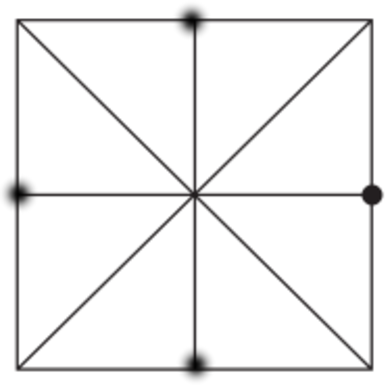
\includegraphics[scale=.3]{../octave/1.pdf}
\item
Stabilizer is $\{R_0,D_+\}$\\
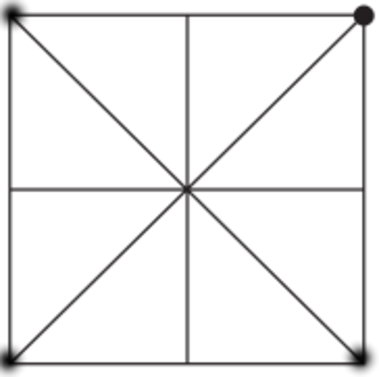
\includegraphics[scale=.3]{../octave/2.pdf}
\item
Stabilizer is $\{R_0,H\}$\\
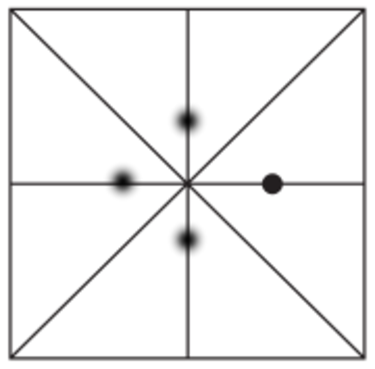
\includegraphics[scale=.3]{../octave/3.pdf}
\item
Stabilizer is $\{R_0\}$\\
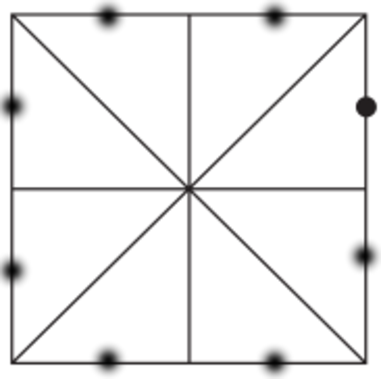
\includegraphics[scale=.3]{../octave/4.pdf}
\item
Stabilizer is $\{R_0\}$\\
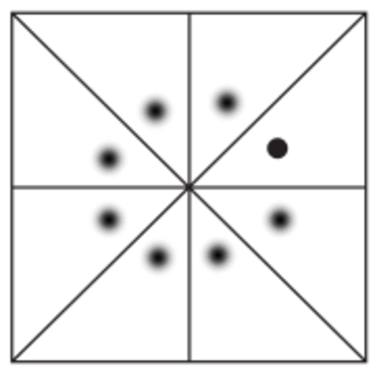
\includegraphics[scale=.3]{../octave/5.pdf}
\item
Stabilizer is $\{R_0\}$\\
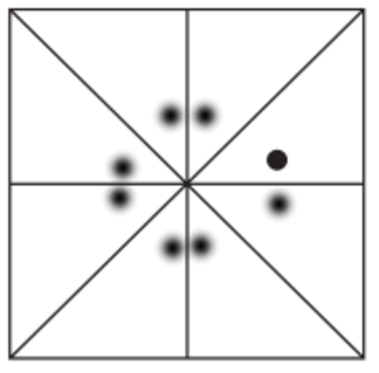
\includegraphics[scale=.3]{../octave/6.pdf}
\end{enumerate}
\end{exercise}






\end{document}